% --- SLIDE 1: PROBLEM IDENTIFICATION & CONTEXT ---
\begin{frame}{Problem Identification \& Context: The Limits of Passive Prostheses}
    \begin{columns}[T]
        \begin{column}{0.45\textwidth}
            \vspace{0.5cm}
            \begin{figure}
                \centering
                \begin{figure}
                    \centering
                    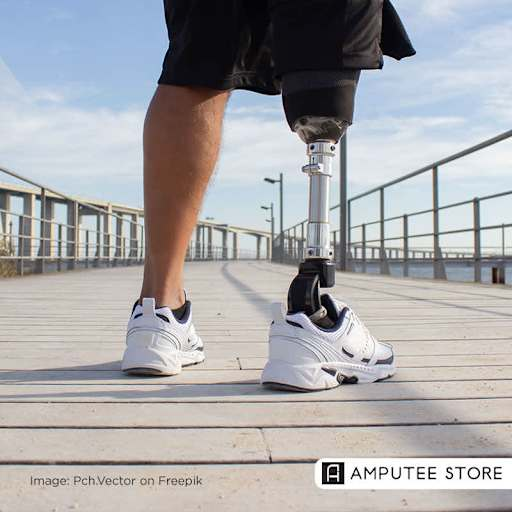
\includegraphics[width=\textwidth, height=3.5cm, keepaspectratio]{image/slide_1.jpg}
                    \caption{{Transtibial amputee with passive prosthesis}}
                \end{figure}
            \end{figure}
        \end{column}
        \begin{column}{0.55\textwidth}
            \vspace{-0.75em}
            \begin{itemize}
                \item \textbf{Context:}
                \begin{itemize} 
                    \item Passive prostheses dominate the market for their reliability and low cost.
                    \item They exhibit a \alert{fixed dynamic response}.
                \end{itemize}
                \item \textbf{Biomechanical Problem:}
                \begin{itemize}
                    \item \textit{Task-invariant response:} fixed stiffness cannot adapt between walking, running, or stair climbing.
                    \item \textit{Terrain-blind mechanics:} no impedance modulation.
                \end{itemize}
                \item \textbf{The Dilemma (Deformability vs. Energy):}
                \begin{itemize}
                    \item \textit{Soft} heel: absorbs impact but dissipates energy.
                    \item \textit{Rigid} heel: returns energy but damages the residual limb.
                \end{itemize}
                \item \textbf{Project Goals:}
                \begin{itemize}
                    \item \textbf{Zero Electronics:} No batteries, no sensors.
                    \item \textbf{Low-Maintenance:} High durability and low cost.
                    \item \textbf{Dynamic Cushioning:} Impact response optimization.
                \end{itemize}
            \end{itemize}
        \end{column}
    \end{columns}
\end{frame}